
\section{Mathematical Background}%
\label{sec:mathematical_background}

We will in this section will we review standardized and well know methods and notations. Generally is the notation followed from \cite[Chapter 1]{pietro2012}.


\subsection{Notation}%
\label{sub:notation}

We will in this report assume $\Omega $ to be a compact and open set in $\mathbb{R} ^{d}$. Let $p \in \mathbb{R} $, $ 1 \le  p \le  \infty$, and  define the space $L^{p}\left( \Omega  \right) $ to be the set of all measurable functions $u: \Omega  \mapsto \mathbb{R} $ such that
$\left\lvert f \right\rvert ^{p}$ is Lebesgue integrable, i.e,

\begin{equation*}
    L^{p}\left( \Omega  \right) = \left\{ u: \Omega \mapsto \mathbb{R}  \mid \int_{\Omega }^{} \left\lvert u \right\rvert ^{p} d \Omega  < \infty  \right\}
.\end{equation*}
Let $u \in L^{p}\left( \Omega  \right) $. We define the integral norm of order $p$ to be \[
\| u \|_{ L^{p}\left( \Omega  \right)  }^{  }  = \left( \int_{\Omega }^{} \left\lvert u \right\rvert ^{p} dx  \right) ^{\frac{1}{p}}.
\]
Since $p=2$ is frequently used in this report, we also define for convenience a compact notation $\| u \|_{ \Omega  }^{  }  = \| u \|_{ L^{2}\left( \Omega  \right)  }^{  } $ .  Recall that $L^{2}\left( \Omega  \right) $ is a Hilbert space if it is equipped with a inner
product of two functions $u,v \in L^{2}\left( \Omega  \right) $ such that
    $
\left( u,v \right) _{\Omega } = \left( u,v \right) _{L^2\left( \Omega  \right) } = \int_{\Omega }^{} u  v dx.
$
The following definition for derivatives is employed,
\begin{equation}
\label{eq:mixed_derivative}
\partial ^{\alpha  } u = \frac{\partial ^{\left\lvert \alpha  \right\rvert } u}{ \partial ^{\alpha _{1} } x_{1} \partial ^{\alpha _{2}} x_{2}  }, \quad \text{for } \alpha=\left( \alpha _{1}, \alpha _{2} \right) \text{ and } f \in C^{\left\lvert \alpha  \right\rvert }
\left( \Omega  \right)
.\end{equation}
For $d$ dimensions of order $k$ we define the multi-index $\alpha  = ( \alpha _{1}, \ldots, \alpha _{d})  $ with the absolute value $\abs{ \alpha  } = \sum_{i=1}^{d}  \alpha _{i} = k $ s.t.
\[
\partial ^{\alpha} u = \frac{\partial ^{ \alpha_{1}  }  } {\partial^{} x_{1}^{\alpha _{1}}  } \ldots \frac{\partial ^{ \alpha_{d}  }  } {\partial^{} x_{d}^{\alpha _{d}}  } u
\]

  Let $m\ge 0$ be an integer and let $1 \le  p \le  \infty$ be a real number. Then the Sobolev space $H^{m}( \Omega ) $ are defined by
\[
H^{m}\left( \Omega  \right) = \left\{ u \in L^{2}\left( \Omega  \right)  \mid  \partial ^{\alpha } u \in L^{2}\left( \Omega  \right)  \forall \alpha : \left\lvert \alpha  \right\rvert  \le m \right\}.
\]
Equipped with the inner product for $u,v \in H^{m}\left( \Omega  \right) $, \[
    \left( u,v \right) _{H^{m}\left( \Omega   \right) } = \sum_{\left\lvert \alpha  \right\rvert  \le  m}^{}  \int_{\Omega }^{} \partial ^{\alpha } u \partial ^{\alpha } v dx,
\]
with the corresponding norm
$
\| u \|_{ H^{m}\left( \Omega  \right)  }^{2  }  =  \| u \|_{ L^{2}\left( \Omega  \right)    }^{2} + \sum_{k = 1}^{m}  \left\lvert u \right\rvert ^{2} _{  H^{k}\left( \Omega  \right) }.
$
Here the seminorm is defined such that, $ \left\lvert u \right\rvert _{H^{k}( \Omega  ) }^{2} =  \sum_{\left\lvert \alpha  \right\rvert  = k}^{} \| \partial ^{\alpha }u \|_{ \Omega  }^{ 2 }  .
$
We will often use the shorthand notation $ \| u \|_{ k, \Omega  }^{  } = \| u \|_{ H^{k}( \Omega)  }^{  } $ and $ \abs{ u }_{ k, \Omega  }^{  }  = \abs{ u }_{ H^{k}( \Omega)  }^{  }$.

Given the context of Sobolev spaces, we consider the functions $ u \in H^{2}( \Omega )$ and $ v \in H^{1}( \Omega )$. We can denote Greens theorem, which links integrals over a volume and its boundary, as follows,
\[
( \Delta u, v) _{\Omega } = -( \nabla u, \nabla v)_{\Omega } + ( u, \partial _{n}v)_{\Gamma }
\]
This identity serves as an essential tool for the calculations done.



\subsection{Computational Domains}%
\label{sub:computational_domain}
Assume that $\Omega \subset \mathbb{R} ^{d} $ is a compact set with a boundary  $\Gamma $. In standard FEM methods a key assumption is that the set $\Omega $ is a polyhedra. This is useful since a polyhedra can be fully covered by a collection of polyhedra and, hence, motivating us to define a fitted mesh.
We define a fitted mesh $\mathcal{T} $ of the domain $\Omega $ to be a collection of disjoint polyhedra $\left\{ T \right\}  $ forming a partition of $\Omega $ s.t $\overline{\Omega } = \bigcup _{T \in \mathcal{T} } T $, for illustration see Figure
\ref{fig:domain_mesh}.
Here we say that each $T \in  \mathcal{T} $ is a mesh element or an element.
The mesh size is defined as the maximum diameter $h := h_{max} $ of any polyhedra in the mesh $\mathcal{T} = \left\{ T \right\}  $, that is, $ h_{max} = \max_{T \in \mathcal{T} }  h_{T}$ s.t.
$h _{T}  = \mathrm{diam}\left( T \right)   = \mathrm{max}_{x_1, x_{2} \in T} \ \mathrm{ dist }(x_{1}, x_{2})$
Hence, motivating us to use the notation $\mathcal{T} _{h}$ for a mesh $\mathcal{T} $ with size $h$.

For simplicity will we restrict ourself to simplicial and quadrilateral elements.
A mesh $\mathcal{T}_{h}$ in $ \mathbb{R} ^{d}$ is said to be matching if
for all neighbouring elements $T_{1}, T_{2} \in \mathcal{T} _{h}$ such that the intersection $T_{1} \cap T_{2} $ is a manifold of dimensions $( d-1)$, then $T_{1} \cap T_{2} $ a entire facet of both $T_{1}$ and $T_{2}$.

Let the chunkiness parameter $c_{T} := h_{T}/r_{T}$, where $r_{T}$  is the largest ball that be inscribed inside a element $T \in \mathcal{T}_{h} $.
A mesh is said to be shape regular if $c_{T}\le  c$ is independent of $T$  and $h$. We also say that the mesh is quasi-uniform only if it is shape regular and $h_{\mathrm{ max }} \le  c h_{\mathrm{ min }}$.
For a more complete description of meshes, see \cite[Chapter 8]{ErnGuermond2021}.

In this thesis will we assume that a mesh $\mathcal{T}_{h} $ is matching, shape regular and quasi-uniform unless specified.
 The fact that the mesh is conform makes is a useful property since the interface between mesh elements has come into contact in the sense
that it is either a vertex or a facet. This with the combination of shape regularity and quasi-uniformity is a major key to prove important inequalities in broken Sobolev spaces \cite[Chapter 1.4.1]{pietro2012}. Hence, the assumptions are very handy when proving convergence.


Let $\mathcal{T}_{h}  = \left\{ T \right\} $ be a mesh of $\Omega \subset  \mathbb{R} ^d $ consisting of polygons $T \in \mathbb{R} ^{d}$.
The set of all facets is the union of external and internal facets, $\mathcal{F} _{h} = \mathcal{F} ^{ext}_{h} \cup \mathcal{F} _{h}^{int} $, where each are defined by
\[
            \mathcal{F}^{int} _{h}  = \left\{ F=T^{+}\cap T^{-}  \mid  T^{+}, T^{-} \in \mathcal{T}_{h}  \right\} \text{ and }
            \mathcal{F}^{ext} _{h}  = \left\{ F= \partial T \cap \partial \Omega    \mid  T  \in \mathcal{T}_{h}  \right\}.
\]
Assume $T^{+} \neq T^{-}$ . Next, we define the following normal vectors.
\begin{enumerate}[label=\arabic*)]
    \item We define $ n= n  _{\partial T}$ to be unit outward normal on $\partial T$ for each $T \in \mathcal{T}_{h} $
\item Let $F \in \mathcal{F }^{int} _{h}$. We define $n$ to be the facet normal $ n =  n _F = n | _{\partial T^{+}} $  from $T^{+}$ to $T^{-}$, illustrated in Figure \ref{fig:normal}. \red{Ask Andre about his comment here.}
 \item Let $F \in \mathcal{F} ^{ext}_{h}$. Then we define the facet normal $n | _{F} = n | _{\partial T} $ to be the unit outward normal.
\end{enumerate}
Please note that we for convenience employ the notation $n$ when it is clear what entity the normal is associated with.

    Let $v\in L^2( \Omega ) $ be a scalar function on $\Omega$ with a corresponding shape regular and quasi-uniform mesh $\mathcal{T}_{h} $. We will use the following definitions.
    \begin{enumerate}[label=\arabic*)]
        \item Let $F \in \mathcal{F}^{int} _{h}$ and $v^{\pm}| _{F} = \lim_{t\to 0^{+}} v( x \mp tn)   $ for $x \in F$. We define the mean as $\mean{ v} |_{F} = \frac{1}{2} (v^{+}_{F} + v^{-}_{F})   $ and the jump as $\jump{v}|_{F} =  v^{+}_{F} - v^{-}_{F} $.
        \item Let $F \in \mathcal{F}^{ext} _{h}$ and let $ v( x) =  v(x)|_{F} $ for  $x \in F$.
We define the mean as $\mean{ v} |_{F} = v    $ and the jump as $\jump{v}|_{F} = v$.

    \end{enumerate}
    To simplify will we use the notation $\mean{ v } = \mean{ v }|_{F}    $ and $\jump{ v } = \jump{ v }| _{F}    $ for all $F \in \mathcal{F} _{h}$.
    Remark that if we have two functions $u,v$, for which $u^{\pm}( x) $ and $v^{\pm}( x) $ are defined, then the following identity holds $  \jump{ uv }    = \jump{ u }   \mean{ v }    + \mean{ u }  \jump{ v }$ along all facets $ \mathcal{F}_{h} $ associated with the
    triangulation $\mathcal{T} _{h}$.


\begin{figure}[h!]
\centering
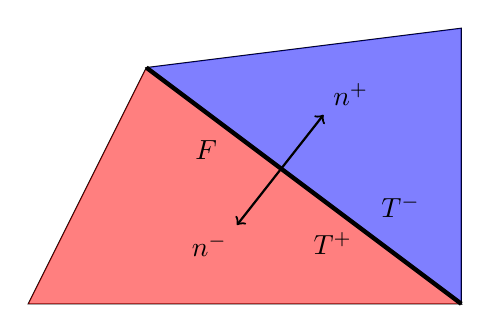
\begin{tikzpicture}[scale=1]
\coordinate (A) at (-1.5, -0);
\coordinate (C) at (0,3);
\coordinate (B) at (4,0);
\coordinate (D) at (4,3.5);

\draw (A) -- (B) -- (C) -- cycle;
\draw (B) -- (C) -- (D) -- cycle;
\fill[red, opacity=0.5] (A) -- (B) -- (C);
\fill[blue, opacity=0.5] (B) -- (C) -- (D);
\draw[ultra  thick] (C) -- (B);

\coordinate (Tm) at (3.6,1.5);
\coordinate (Tp) at (2.0, 0.5);
\coordinate (e) at (0.5, 2.2);
\node[below left] at (Tm) {$T^{-} $ };
\node[above right] at (Tp) {$T^{+}$ };
\node[below right] at (e) {$F$ };

\coordinate (start) at (1.7, 1.7);
\coordinate (endPlus) at (2.25, 2.4);
\coordinate (endMinus) at (1.15, 1.0);

\draw [->, thick] (start) -- (endPlus);
\node[above right] at (endPlus) {$n^{+}$};

\draw [->, thick] (start) -- (endMinus);
\node[below left] at (endMinus) {$n^{-}$};

\end{tikzpicture}

\caption{Facet $F \in \mathcal{F}_h^{int} $ shared by the triangles $T^{+}, T^{-} \in \mathcal{T}_{h} $ and the normal unit vector $n^{+}$ and $n^{-}$. If we pick $T=T^{+}$ and want to evaluate the normal vector $n$ along a facet $F$, then we define $n = n  \mid _{F} = n^{+}$.}
    \label{fig:normal}
\end{figure}



\subsection{Broken Sobolev spaces}%
\label{sub:broken_sobolev_spaces}

In this work will we compute norms on discontinuous elements, thus, it will be necessary to define broken Sobolev spaces.
Let $\mathcal{T}_{h} $ be a mesh and some integer $m\le n$. Then we define the broken Sobolev space to be \[
    \begin{split}
H^{m}( \mathcal{T}_{h} ) & := \left\{ v \in L^2( \Omega )  \mid \ v|_{T} \in H^{m}( T) \quad     \forall T \in  \mathcal{T} \right\}\\
        L^{2}( \mathcal{F}_{h} ) &:= \left\{ v \in L^2( \mathcal{T}_{h}  )  \mid   \ v|_{F} \in L^{2}( F)  \quad  \forall F \in  \mathcal{F}_{h}   \right\}.
    \end{split}
\]
This motivates us to define broken Sobolev norms and inner products using a summation over mesh elements. That is,
\[
 \| v \|_{H^{m}( \mathcal{T}_{h} ) }^{2} = \sum_{T \in  \mathcal{T}_{h} }^{} \| v  \|_{ H^{m}( T ) }^{2  } \quad \text{ and } \quad
 (v ,w )_{H^{m}( \mathcal{T}_{h} ) }^{} = \sum_{T \in \mathcal{T} _{h}}^{} (v ,w )_{ H^{m}( T ) }^{  } .
\]
As expected we use the notation,  $\| v \|_{\mathcal{T}_{h}} =  \| v \|_{L^{2}( \mathcal{T}_{h} ) }$ and  $(v ,w )_{ \mathcal{T}_{h} }^{} = (v ,w )_{L^2( \mathcal{T}_{h} ) }^{} $.
That is,
\[
 \| v \|_{H^{m}( \mathcal{F}_{h} ) }^{2} = \sum_{F \in  \mathcal{F}_{h} }^{} \| v  \|_{ L^{2}( F ) }^{2  } \quad \text{ and } \quad
 (v ,w )_{L^{2}( \mathcal{F}_{h} ) }^{} = \sum_{T \in \mathcal{F} _{h}}^{} (v ,w )_{ L^{2}( F ) }^{  } .
\]
And again, we often use the more compact notation $\| v \|_{\mathcal{F}_{h}} =  \| v \|_{L^{2}( \mathcal{F}_{h} ) }$ and  $(v ,w )_{ \mathcal{F}_{h} }^{} = (v ,w )_{L^2( \mathcal{F}_{h} ) }^{} $.
A very useful lemma when working on estimates on broken Sobolev spaces is that a if a function is continuous, then the jump between the mesh elements is zero. A function $ v \in  H^{1}( \mathcal{T}_{h} ) $ belongs to $ H^{1}( \Omega )  $ if and only
if $ \jump{ v }   = 0 \text{ for }  F \in \mathcal{F}^{int}_{h}$.



\subsection{Useful inverse estimates}%
\label{sub:useful_inverse_estimates}

Some useful inequalities.
\begin{enumerate}[label=(\roman*)]
    \item Cauchy-Schwarz inequality
    \[
     \| ab \|_{  }^{  }  \le \| a \|_{  }^{  } \| b \|_{  }^{  }
    \]
    \item Youngs $\varepsilon $-inequality
        \[
            2ab \le \varepsilon a^2+ b^2 \frac{1}{\varepsilon }
        \]
    \item  First order inverse inequality  \[
    \| \partial _{n} v \|_{ F   }^{  } \le  C_{I} h_{}^{-\frac{1}{2}} \| \nabla v \|_{  T}^{  }
    \]
    \item Second order inverse inequality
        \[
            \frac{1}{h}\| \partial _{nn}  v_{h} \|_{F   }^{2  }  \le C_{j} \| D ^2 v_{h} \|_{ \mathcal{T} _{h} }^{ 2 }   \\
        \]
    \item General inverse inequality.
    Let $\alpha = ( \alpha _{1}, \ldots, \alpha _{N}) $ and $\beta = ( \beta _{1}, \ldots, \beta _{N} ) $.
    Assume $u \in H^{\abs{ \beta  }  }( T) $. The following inverse inequalities hold.
    \[
        \begin{split}
        \| \partial ^{\alpha } u \|_{T  }^{  } & \lesssim h^{ - \abs{ \beta  }  } \| \partial ^{\alpha - \beta } u \|_{T }^{  } \\
        \| \partial ^{\alpha }_{n} u  \|_{F  }^{  } &\lesssim h^{-\frac{1}{2}  } \| \partial ^{\alpha } u \|_{T }^{  }
        \end{split}
    \]
    For a full triangle we have \[
    \| v \|_{ \partial T }^{  } \lesssim h_{T}^{-\frac{1}{2}} \| v \|_{ T }^{  } + h_{T}^{\frac{1}{2}} \| \nabla v \|_{ T }^{  }
    \]
\end{enumerate}




\subsection{Lax-Milgram lemma}%
\label{sub:lax_milgram_lemma}


\begin{definition}[Linear bounded functional]
    \label{def:linear_function}
Let $X$ be a Hilbert space. Furthermore, we define the dual space the be the space of linear and bounded functionals $F: X  \mapsto \mathbb{R} $, i.e., \[
X'  =
\left.
\begin{cases}
F: X  \mapsto \mathbb{R} \text{ s.t. }\forall v,w \in X, \forall a,b \in \mathbb{R} \text{ and } C> 0 \text{ is }   \\
  F\left( \lambda v + \mu w  \right) = \lambda F(v) + \mu F(w) \text{ and } \left\lvert F\left( v \right)  \right\rvert \le C \| v \|_{ X  }^{  }
\end{cases}
  \right\}
\]
% and we equip it with the functional norm,  \[
%     \| F \|_{ \mathcal{V} ^{*} }^{  } = \sup_{v \in \mathcal{V}   } \frac{\left\lvert F\left( v \right)  \right\rvert }{\| v \|_{ \mathcal{V}  }^{  } }.
% \]
% \todo[inline]{ Maybe write it in terms of $\mathcal{L} $ definition instead. Might need to do some dive into functional analysis books. Anyhow, I am not happy with this definitionin context with the rest of the subchapter.}
\end{definition}

% \begin{definition}[Bilinear bounded functional]
%     \label{def:bilinear_function}
%     Write definitions of a bilinear bounded operator
% \end{definition}

\begin{problem}[Abstract linear problem]
    \label{def:abstract_linear_problem}
    Assume $X$ and $Y$  to be two Hilbert spaces. Let the vector space $\mathcal{L}( X,Y)  $ be all linear bounded operators spanned from $X$ to $Y$. We define the abstract linear problem as follows; find $u \in X$ s.t. \[
    a( u,v)  = l(v ) := \left<f,v \right>_{X' , X}  \forall v \in X
    \]
    Where $a \in  \mathcal{L} ( X \times X,\mathbb{R} ) $ is a bounded linear form and $f \in X':= \mathcal{L} ( X,\mathbb{R} )  $ is a bounded linear form. Here we denote $\left<\cdot ,\cdot  \right>_{X' .X} $ as the duality pairing between $X' $
    and $X $.

\end{problem}


\begin{definition}[Coercivity]
    \label{def:coercivity}
    Let $X$ be a Hilbert space and let $a \in  \mathcal{L} ( X \times  X,\mathbb{R} )  $. Recall that the bilinear form $a$ is coercive on $X$ if there exists an constant $C > 0 $ s.t. \[
     a( v,v) \ge  C \| v \|_{ X }^{  } \quad  \forall v \in  X
    \]
\end{definition}


\begin{lemma}[Lax-Milgram]
    \label{def:lax-milgram}
    We say that the abstract linear problem \ref{def:abstract_linear_problem} is well-posed if $a$ is coercive. Moreover, the following a priori estimate holds true.\[
    \| v \|_{ X }^{  } \le \frac{1}{C} \| f \|_{ X'  }^{  }
    \]
\end{lemma}
\begin{proof}
    The problem can easily be proved using a special case of the Banach–Nečas–Babuška theorem. See \cite[Lemma 1.4]{pietro2012}
\end{proof}



\subsection{Finite element method}%
\label{sub:finite_element_method}


The finite element method (FEM) is a numerical method to solve partial differential equation by finding an approximation of the Problem \ref{def:abstract_linear_problem}.  Let $X_{h}$ be a finite-dimensional (polynomial) approximation space on the mesh
$\mathcal{T} _{h}$. We say that a method is conform if $X_{h}\subset X $ and non-conform if $X _{h} \not\subset X$. We define the approximate problem as follows.
\begin{problem}[The approximate problem]
    \label{def:approx_problem}
    Find  $u \in X_{h}$ s.t. \[
    a_{h}(u,v ) = \left<f,v \right>   \forall v \in X_{h}
    \]
\end{problem}

We denote the functional $a_{h}: X_{h} \times X_{h} \to \mathbb{R} $ as an consistent approximation of $a: X \times X \to \mathbb{R} $, and similarly for the right-hand side.


\begin{definition}[Broken polynomial spaces]
    Let $\mathcal{T}_{h} $ be a mesh of $\Omega \in \mathbb{R} ^{d} $. Let $\mathcal{P}^{k}(T) $ be the space of all polynomials of degree $k$ in the mesh element $T$. We define the broken polynomial space as \[
    \mathcal{P}^{k} ( \mathcal{T}_{h} ) := \left\{ v \in L^2( \Omega )  \mid  v|_{T} \in \mathcal{P}^k( T) \quad  \forall T \in  \mathcal{T}_{h}   \right\}.
    \]
\end{definition}





